\documentclass[a4paper, 12pt, oneside]{article}

%****************packages**************
\usepackage[french]{babel}
\usepackage[T1]{fontenc}
\usepackage{setspace}
\usepackage{hyperref}
\usepackage[top=2.5cm, bottom=2.5cm, left=2.5cm, right=2.5cm]{geometry}
\usepackage{graphicx}
\usepackage{amssymb}
\usepackage[squaren,Gray]{SIunits}
\usepackage{tabularx}
\usepackage{float}
\usepackage{comment}
\usepackage{layout}
\usepackage{pifont}
\usepackage{enumitem}
\usepackage{multicol}
\usepackage{wasysym}
\usepackage{amssymb}
\graphicspath{ {./images/} }
\frenchbsetup{StandardLists=true}
\usepackage{epstopdf}
\epstopdfsetup{outdir=images/converted_to_pdf} % Dossier de sortie des images converties
\usepackage{fancyhdr}
\usepackage{graphicx,lipsum,wrapfig}
\usepackage{csquotes}
\usepackage{biblatex}
\usepackage{marvosym}
\usepackage{booktabs}
\usepackage[table,xcdraw]{xcolor}
\addbibresource{sources.bib}

% fichier perso (à adapter suivant le rapport)
%%%%%%%  Constantes (à changer) %%%%%%%%


\newcommand{\nomAuteur}{Zemrani Nadir \& Cohu Rémi \& Küng Jonathan \& Baechler Stéphanie \& Marques Antony}

\newcommand{\titre}{Diabète Game}

\newcommand{\classe}{607-3}

\newcommand{\departement}{Informatique de gestion (HEG)}

\newcommand{\cours}{646-2 - Choix d'école}

\newcommand{\unitp}[1]{\ensuremath{\, \mathrm{#1}}}



%\setlength{\headheight}{27.06pt}
\pagestyle{fancy}

% Entête :
\fancyhead{} %remove header
\renewcommand{\headrulewidth}{0pt} % remove line

% Pied de page
\fancyfoot{} % clear all footer fields
\renewcommand{\footrulewidth}{0.5pt}
\fancyfoot[R]{\scriptsize Page \thepage}
\fancyfoot[L]{\scriptsize HEG-VS | \nomAuteur }

%****************Document****************
\begin{document}
%\layout
\begin{titlepage}
  \vfill

  \begin{center}
    
\includegraphics[height=2cm]{images/logoHevs.png}
    \hfill
    
\includegraphics[height=2cm]{images/logo_hes-so.eps}
  \end{center}

  \vfill

  \begin{center}
    \Large Guide utilisateur\\
    \huge  \textbf{\titre\\}
  \end{center}

  \begin{center}
    \begin{tabular}{l l}
      Département : & \departement \\
      Module :      & \cours
    \end{tabular}
  \end{center}

  \vfill

  \begin{center}
    \begin{tabular}{l l l l}
      Auteurs :     & Zemrani Nadir            \\
                    & Cohu Rémi                \\
                    & Küng Jonathan            \\
                    & Baechler Stéphanie       \\
                    & Marques Antony           \\
      Professeurs : & Cotting Alexandre        \\
                    & Schumacher Michael Ignaz \\
      Classe :      & \classe                  \\
      Date :        & \today
    \end{tabular}
  \end{center}

  \vfill

\end{titlepage}
\tableofcontents
\thispagestyle{empty}
\newpage

\thispagestyle{empty}
\listoffigures
\listoftables
\newpage
\pagenumbering{arabic}

%============================================================
%****************Intro*******************

\section*{Introduction}
%\label{chap:Introduction} je sais plus à quoi ça sert donc comment au cas ou besoin
\addcontentsline{toc}{section}{Introduction}

Ce projet d'étudiant.e.s est réalisé dans le cadre du module 642-6 Choix d'école de la HES-SO Valais Wallis pour le bachelor en Informatique de Gestion.






%============================================================
%****************Jeu*******************

\section*{Le jeu}
\addcontentsline{toc}{section}{Le jeu}


%============================================================
%****************Sac à dos*******************

\subsection*{Le sac à dos}
\addcontentsline{toc}{subsection}{Le sac à dos}

L'utilisateur a la possibilité d'afficher le contenu du sac à dos en cliquant sur l'icône sac en bas à droite de l'écran.


%============================================================
%****************Onglet 2 planning*******************

\subsubsection*{Planning de la journée}
\addcontentsline{toc}{subsubsection}{Planning de la journée}

Le second onglet du menu du sac à dos est le planning. En cliquant sur cet onglet, l'utilisateur a la possibilité de visualiser son planning de la journée. \\

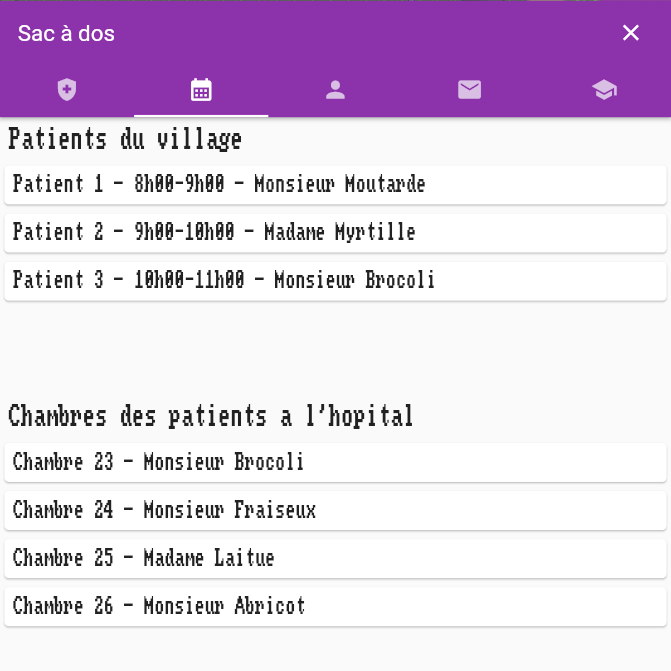
\includegraphics[height=10cm]{images/toolsMenu/planning_screenshot.png}




%============================================================
%*********************Conclusion*****************************

\section*{Conclusion}

\addcontentsline{toc}{section}{Conclusion}

\end{document}
